%%%%%%%%%%%%%%%%%%%%%%%%%%%%%%%%%%%%
% KTHEEtitlepage_ex.tex
%
% Example of how to use the KTHEEtitlepage package.
% 
% Mats Bengtsson,  7/8 2006
%%%%%%%%%%%%%%%%%%%%%%%%%%%%%%%%%%%%


\documentclass[a4paper]{article}

\usepackage[ireport]{KTHEEtitlepage}

% Packages used in the main document for this particular example:
\usepackage{hyperref}
\usepackage{graphicx}
\usepackage{cite}	



\begin{document}
% Information to appear on the title page:
\ititle{Project Plan}
\isubtitle{A visualization interface for spatial pathway regulation data}
\iauthor{Yang Zhang}
\idate{2018-3-13}

\iaddress{Industrial and Environmental Biotechnology (TIMBM)}
\makeititle

% Everything below is exactly as for a normal document and 
% the layout of that document should not be affected in any
% way by the title page.


\section{Objective}
The main objective of this degree project is to create a web browser-based data visualizer that is able to combine the information from the pathway databases with the data derived from \textit{Spatial Transcriptomics}. The project will be performed with 20 week period, including the course' objectives of project planning, lab working, scientific reporting and oral presentation.

\subsection{Datasets and tools preparation}
This project is an extension of work from a study of previous Spatial Transcriptomics, which provided a data set to quantitative differences of pathway genes presented in multiple tissue sections. The first objective of the project is to study the background and formation of those pathway datasets, understand knowledge on how the ST data was being structured from previous studies.

Secondly, how to code in d3.js and JavaScript need to be learnt as the \textit{d3.js} libraries are highly dependable for data visualization and JavaScript(Python) can be helpful for interface development.


\subsection{Data visualization}
A major objective for this thesis project is to present the Spatial Transcriptomics data in a more intuitive way. The idea is to first create an image that illustrates the level of pathway expression of a certain tissue. This type of image should be semi-transparent so it can overlaid with its histological section. Secondly, a sunburst diagram should be plotted which represents the hierarchical nature of the pathways as well as displays information on how relevant those pathways are. 

\subsection{Interface Development}
To present the previous data visualization works in an easy-navigate way, we aim at designing a web-browser-based interface by using JavaScript and Python. We  will embed the D3 code into HTML's script part. The requirement is also to develop the tool to be easy in interact, hopefully facilitating the user's exploration of ST data in order to increase the usefulness of Spatial Transcriptomics information \cite{ST}.

\subsection{Write a master's thesis and hold a presentation}
The purpose of thesis and oral presentation are to convey the project into a form that is communicable to others. The master's thesis and the presentation should provide a full and correct picture of the project and its derivatives. 


\section{Background}
A biological pathway is a series of actions among molecules in a cell that leads to a certain product or a change in a cell.\cite{NHGRI} Such a pathway can trigger the assembly of new molecules, such as a fat or protein. Pathways can also turn genes on and off, or spur a cell to move.

In any organism, there is a large number of biological pathways , i.e. sets of of related biomolecules, which together conducts different functions of its cells. There are multiple pathway databases such as \textit{KEGG}\cite{KEGG}, \textit{Gene Ontology} \cite{GENE} and \textit{Reactome} \cite{RE}. These pathway databases are normally formed with a map of moleculalr interaction/reaction network diagram, which representing knowledge on molecular interaction, reaction and relation networks of different organisms \cite{KEGG} (e.g. Metabolism, Human Diseases, Drug Development).

Although the definition of pathways may vary among databases, the concept that genes can control the activities among different pathways has been established. However when the study focus on specific tissue sections and their cells, the questions has been raised: is the transcriptoms in the section yield the result of regulation of pathways? Based on those pathways databases, correlated with the method \textit{Spatial Transcriptomics} is the way to solve the problem.

Spatial Transcriptomics is a method that allows visualization and quantitative analysis of the transcriptome in individual tissue sections. By probing the histological sections at different locations, arrayed with oligonucleotides containing positional bar-codes, it is possible to generate cDNA libraries with precise positional information for RNA-seq. This provides transcriptome data in a versatile format for bioinformatics analyses of gene expression within the tissue context. In this case, the Spatial Transcriptomics generate the result shows the qualities of genes regulating the pathways in tissues. Those results will be valuable for further data visualization studies \cite{ST}.

\textit{Javascript} (JS): is a interpreted programming language, which also characterized as dynamic, weakly typed, prototype-based language. JavaScript commonly used to make webpages interactive and provide online programs  \cite{JA}. The majority of websites employ it, and all modern web browsers support it without the need for plug-ins, thus it fit the usage to create web-browser base interface for this project. 

\textit{D3.js} is a JavaScript library for manipulating documents based on data. D3 is able to bring data to life using HTML and SVG. D3 is emphasis on web standards, which gives the full capabilities of modern browsers to combine visualization components and a data-driven approach to Document Object Model(DOM) manipulation, in order to apply data-driven transformations to the document. For example, one use D3 to generate an HTML table from an array of numbers. Or, use the same data to create an interactive SVG bar chart with smooth transitions and interaction.

\section{Work Breakdown Structure}
A work breakdown structure (WBS) is a hierarchical breakdown of large activities into smaller and more comprehensible units. The WBS of the degree project is presented in Figure 1. 

\begin{figure}[h]
	\centering
	\includegraphics[scale=0.4]{WBS.pdf}
	\caption{Work breakdown structure}
\end{figure}



\section{Milestones}
\begin{enumerate}
  \item \textbf{Basic tools prepared, Instructions read} - When reach this milestone, it means all pre-study works about \textit{d3.js}, Javascript and database backgrounds' study will be finished. Also the tools preparation such as github and local server set up can be completed. Major coding works will begin after this milestone. 
  \item \textbf{Data visualization complete} - That will be a relatively loose milestone, once data visualization codes been written,  it means a basic pathway expression visualizer will be created. However, code will have to modified to meet the adjust of the requirement from the subsequence working packages.
  \item \textbf{Half-time meeting} - The second version of the project plan will be finished before the half-time meeting. Categorized problems encountered in the stage that need to be overcomed. There after formed a matured project structure and handled to examiner and supervisor.
  \item \textbf{Interface created} 
  \item \textbf{Data modification finished} -  main coding job of the project is completed and a primitive program should deliver.
  \item \textbf{Program verified and evaluation complete} - A final version of program should be carried out, start writing master thesis afterwards.
  \item \textbf{Final version of master’s thesis finished} – can subsequently be handed in. 
  \item Presentation - final milestone.
\end{enumerate}

\section{Time plan}

A Gantt chart based on the Work breakdown structure which also including milestones and deadlines presented in Figure 2. It shows an approximated time estimates for the whole project.

\begin{figure}[h]
	\centering
	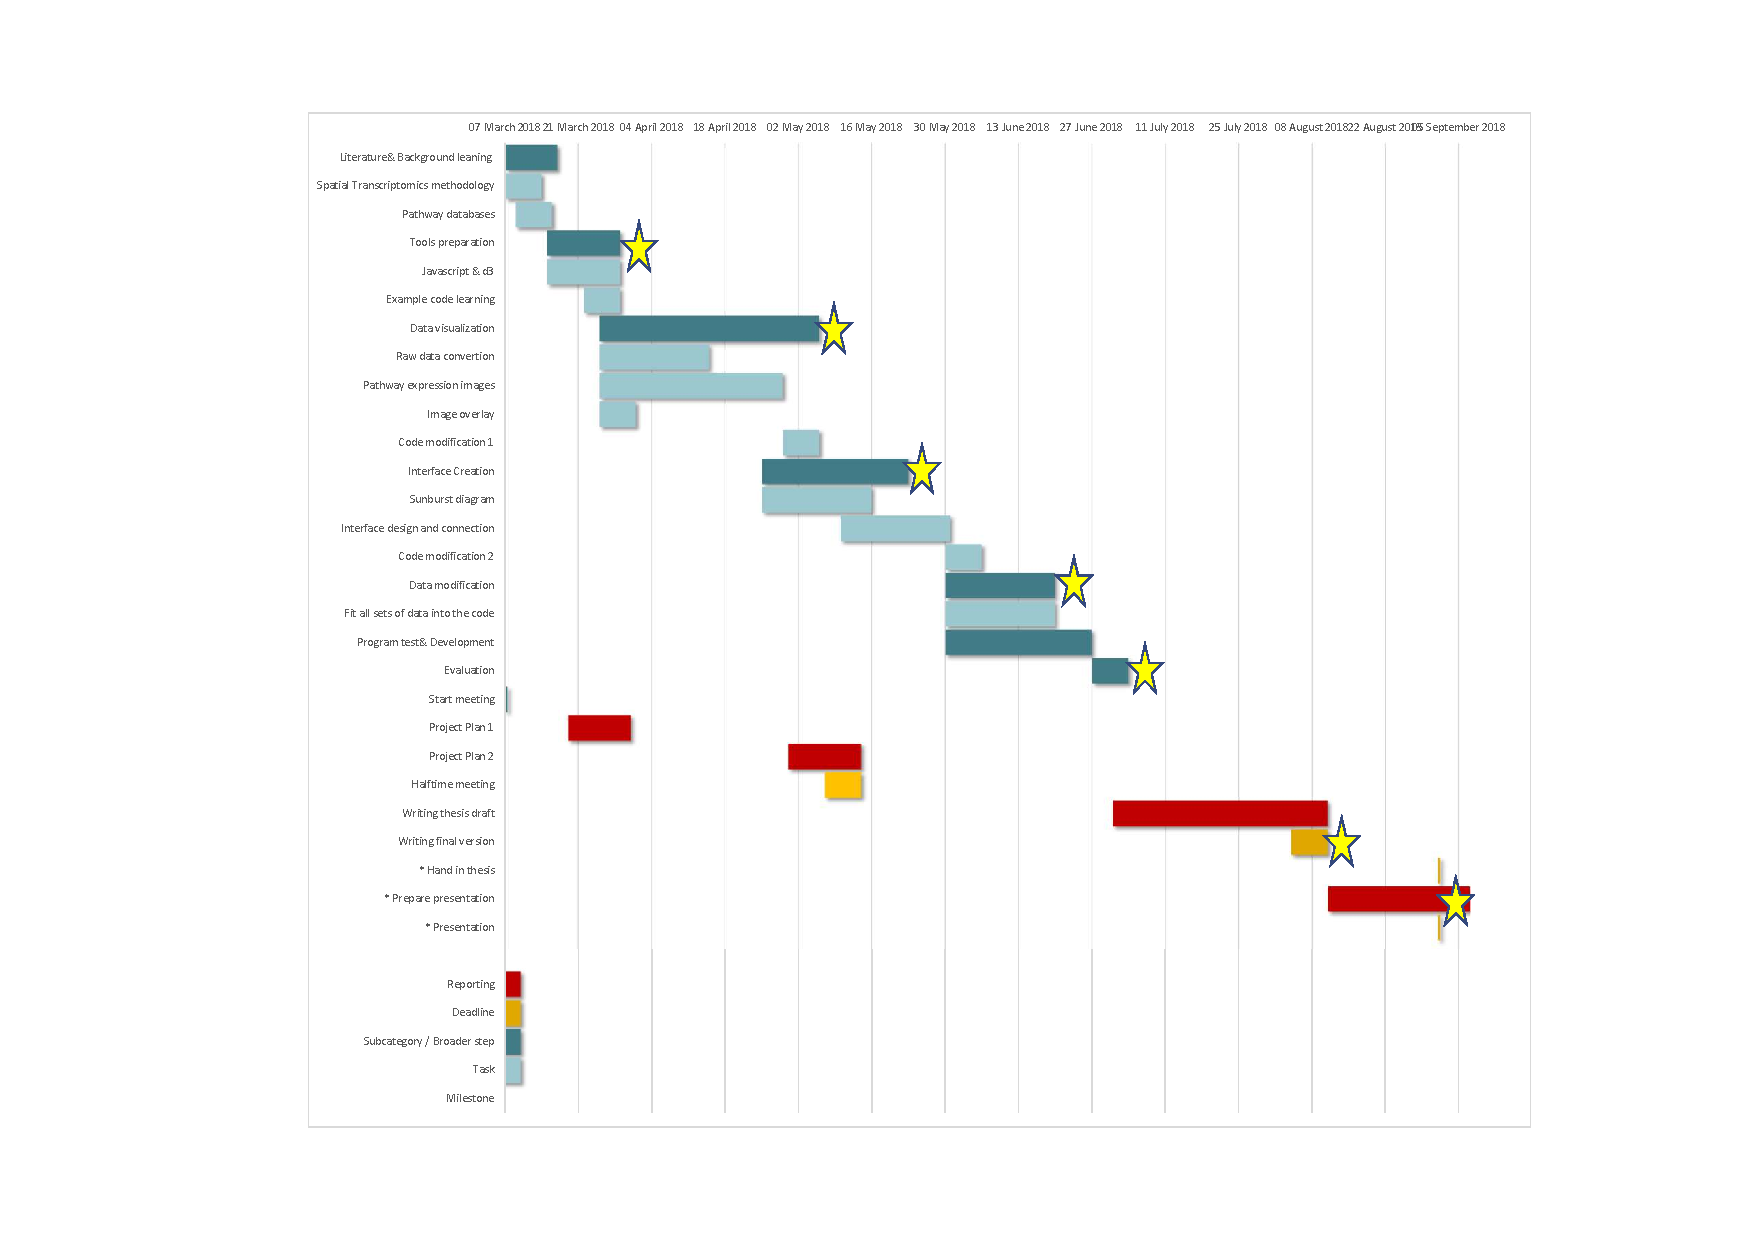
\includegraphics[width=\textwidth]{Gannt.pdf}
	\caption{Gannt time table, * the date to hand up thesis and hold presentation is during week 19,20 according to the project schedule, the real data may vary due to the summer break. }
\end{figure}


\section{Specification (in MoSCoW)}
The MoSCoW structure (Must Have, Should Have, Could Have, Won't Have this time) is used to prioritise tasks related to the project.

Must 
\begin{itemize}
  \item Successful convert the ST data(csv) into visualized pathway expression image.
  \item Overlaid the pathway expression images into histological sections.
  \item Create a visualizer interface that fits required sets of data.
  \item Project planning. 
  \item Write master’s thesis. 
  \item Opposition
  \item Oral Presentation
\end{itemize}

Should
 
\begin{itemize}
  \item Optimize the code to fit more data sets.
  \item Successful handle the connection and shifts between sunburst diagram and overlaid images.  
  \item Create a csv data auto converting program
\end{itemize}

Could 
 
\begin{itemize}
  \item Develop the interface to become user friendly and easy navigating. 
  \item Try to create a images zoom-able program.
\end{itemize}

Will not
 
\begin{itemize}
  \item A deep understand of Spatial Transcriptomics.
  \item A strategy to quantitatively judge the quality of pathway expression in tissues.
\end{itemize}


\clearpage
\bibliography{plan}{}
\bibliographystyle{numeric}


\end{document}
